\documentclass{beamer}
\mode<presentation>
{
  \usetheme{default}      % or try Darmstadt, Madrid, Warsaw, ...
  \usecolortheme{default} % or try albatross, beaver, crane, ...
  \usefonttheme{default}  % or try serif, structurebold, ...
  \setbeamertemplate{navigation symbols}{}
  \setbeamertemplate{caption}[numbered]
} 

\usepackage[english]{babel}
\usepackage[utf8x]{inputenc}

\usepackage{geometry}

\usepackage{subcaption}
\usepackage{amsmath}
\usepackage{mathtools}
\DeclarePairedDelimiter\abs{\lvert}{\rvert}%
\DeclarePairedDelimiter\norm{\lVert}{\rVert}%

\title[Hacking the Xgboost]{Hacking the Xgboost}
\author{Raul Sanchez-Vazquez}
\institute{Kunumi}
\date{22 June 2018}

\begin{document}

\begin{frame}
  \titlepage
  
\end{frame}

%\begin{frame}{Outline}
%  \tableofcontents
%\end{frame}

\section{Introduction}

\begin{frame}{Introduction}

\begin{figure}
	\centering
	\begin{subfigure}{.45\textwidth}
		\centering
		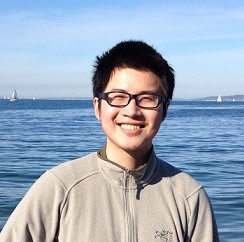
\includegraphics[width=.7\linewidth]{img/Tianqi_Chen}
		\caption{Tianqi Chen}
		\label{fig:sub2}
	\end{subfigure}
	\begin{subfigure}{.45\textwidth}
		\centering
		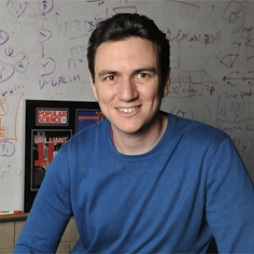
\includegraphics[width=.7\linewidth]{img/Carlos_Guestrin}
		\caption{Carlos Guestrin}
		\label{fig:sub1}
	\end{subfigure}
	\caption{Authors}
	\label{fig:test}
\end{figure}
\end{frame}

\begin{frame}{Introduction}
	Tianqi Chen:
	
	\begin{itemize}
		\item (2013 – Present) Ph.D. Student (University of Washington)
			\begin{itemize}
			\item Social Media and Recommender Systems
			\end{itemize}
		\item (2012 – 2012) Intern (Huawei Noah's Ark Research Lab)
		\item (2009 – 2012) Teaching Assistant (Shanghai Jiao Tong University)
		\begin{itemize}
			\item Compiler
			\item Operating System
			\item Database Management System
			\item Data Mining and Machine Learning in Practice
		\end{itemize}
		\item (2011 – 2011) Visiting Scholar (DERI)
		\begin{itemize}
			\item Information extraction from technology reviews
		\end{itemize}
		\item (2010 – 2013) Master in Computer Science (Shanghai Jiao Tong University)
		\item (2006 – 2010) Bsc Computer Science (Shanghai Jiao Tong University)
	\end{itemize}
	
\end{frame}

\begin{frame}{Introduction}
	Carlos Guestrin:
	
	\begin{itemize}
	\item (2016 – Present) Senior Director of AI and Machine Learning (Apple)
	\item (2012 – Present) Professor of Machine Learning (University of Washington)
	\item (2013 – 2016) Founder $\&$ CEO (NameDato, Inc.)
	\item (2009 – 2012) Co-Founder (Flashgroup)
	\item (2004 – 2012) Associate Professor (Carnegie Mellon University)
	\item (2003 – 2004) Senior Researcher (Intel Corporation)
	\item (1998 – 2003) Ph.D Computer Science (Stanford University)
	\item (1993 – 1998) Mechatronics, Robotics, and Automation Engineering (Universidade de São Paulo)
	\end{itemize}
	
\end{frame}

\begin{frame}{Gradient Boosting}

Dataset:

\begin{equation*}
\mathcal{D} = \{(x_i, y_i)\}
\end{equation*}

Given $n$ examples and $m$ features $\abs{\mathcal{D}} = n$ and $x_i \in  \mathbb{R}^m$

\begin{equation}
	\hat{y_i} = \sum_{k=1}^{K} f_k(x_i), f_k \in \mathcal{F}
\end{equation}

Where $K$ is the number of week learners and $f_k$ is a single week learner drawn from $\mathcal{F}$, which is the space of all possible learners (i.e. decision trees, neural nets, k-neares-neighbors, linear regression, SVM,).
	
\end{frame}

\begin{frame}{Decision Tree}
In the specific case of XGBoost, $\mathcal{F}$ is the space of regression trees (known as CART):

\begin{equation*}
\mathcal{F} = \{f(x) = w_q(x)\}(q: \mathbb{R}^m \rightarrow T, w \in \mathbb{R^T})
\end{equation*}
\begin{itemize}
	\item $q$ represents the structure of each tree that maps to leaf indexes
	\item $T$ is the number of leaves in the tree
	\item $f_k$ corresponds to an independent tree structure $q$ and weights $w$
	\item $w_i$ corresponds to the score in the $i$-th leaf
\end{itemize}

\end{frame}

\begin{frame}{Example of decision tree}
	
\begin{figure}
	\centering
	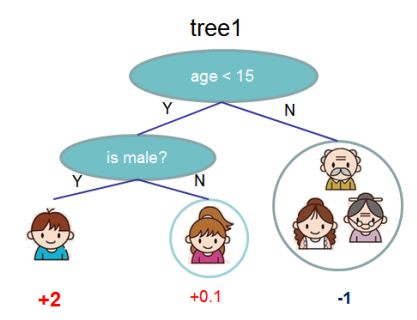
\includegraphics[width=.7\linewidth]{img/tree_example}
	\caption{Tree example}
\end{figure}
\begin{itemize}
	\item $T = 3$
	\item $w = \{w_1, w_2, w_3\} = \{2, .1, -1\}$
	\item $q$ is the tree structure
\end{itemize}	

\end{frame}

\begin{frame}{Loss Function}

	\textbf{Regularized} learning objective:
	
	\begin{equation}
		\mathcal{L}(\phi) = \sum_i l(\hat{y}_i, y_i) + \sum_k \Omega(f_k)
	\end{equation}

	Where:
	\begin{itemize}
			\item $ \Omega(f) = \gamma T + \frac{1}{2} \lambda \norm{w}^2$
			\item The function $l$ must be differentiable
	\end{itemize}

\end{frame}

\begin{frame}{Gradient Tree Boosting}
	
	\begin{itemize}
		\item The tree ensemble cannot be optimized using traditional optimization methods.
		\item For such reasons, the ensemble model is trained in an \textbf{additive manner}
	\end{itemize}
	
	Let $\hat{y}_i^t$ be the prediction of the $i$-th instance at iteration $t$. We will need to add $f_t$ to minimize the following objective:
	
	\begin{equation*}
	\mathcal{L}^{(t)} = \sum_{i=1}^{n} l(y_i, \hat{y}_i^{(t-1)} + f_t(x_i)) + \Omega(f_t)
	\end{equation*}

\end{frame}

\begin{frame}{Newton's Method}

\begin{figure}
\centering
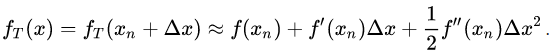
\includegraphics[width=0.7\linewidth]{img/taylor_expansion}
\caption{Newton's method in optimization}
\label{fig:taylor_expansion}
\end{figure}

\begin{figure}
	\centering
	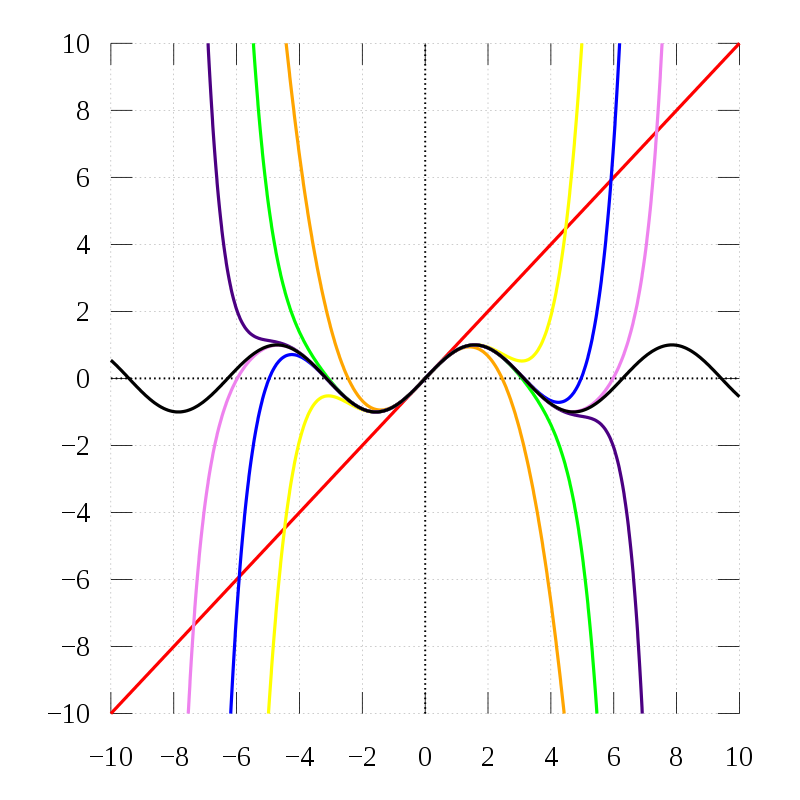
\includegraphics[width=0.5\linewidth]{img/example_approx}
	\caption{Taylor Expansion}
	\label{fig:taylor_expansion}
\end{figure}
\end{frame}

\begin{frame}{Second Order approximation}
	
Regularized objective:

	\begin{equation*}
	\mathcal{L}^{(t)} = \sum_{i=1}^{n} l(y_i, \hat{y}_i^{(t-1)} + f_t(x_i)) + \Omega(f_t)
	\end{equation*}
		
Applying second-order approximation:
	
	\begin{equation*}
	\mathcal{L}^{(t)} \approx 
	\sum_{i=1}^{n} 
	\big[ 
		l(y_i, \hat{y}^{(t-1)}) +
		g_i f_t(x_i) + 
		\frac{1}{2} h_i f_t^2(x_i) 
	\big] +
	\Omega(f_t)
	\end{equation*}

Where
\begin{itemize}
	\item $ g_i = \partial_{\hat{y}(t-1)} l(y_i, \hat{y}^{t-1})$ first gradient on the loss function
	\item $h_i = \partial^2_{\hat{y}(t-1)} l(y_i, \hat{y}^{t-1})$ second gradient on the loss function
\end{itemize}

\end{frame}

\begin{frame}{Simplified Loss}
	
	Simplifying the second-order approximation equation:
	
	\begin{equation}
		\label{eq:simpleloss}
		\tilde{\mathcal{L}}^{(t)} = \sum_{i=1}^{n}
		\big[ 
			g_i f_t(x_i) + \frac{1}{2} h_i f_t^2(x_i)
		\big]
		 + \Omega(f_t)
	\end{equation}
	
	Define $I_j = \{ i | q(x_i) = j \}$ as the instance set of leaf $j$. 
	We can rewrite Eq~\refeq{eq:simpleloss} by expanding $\Omega$:
	
	\begin{equation*}
		\tilde{\mathcal{L}}^{(t)} = \sum_{i=1}^{n}
		\big[ 
		g_i f_t(x_i) + \frac{1}{2} h_i f_t^2(x_i)
		\big]
		+ \gamma T
		+ \frac{1}{2} \lambda \sum_{j=1}^{T} w_j^2
	\end{equation*}
		
\end{frame}

\begin{frame}{Simplified Loss}
	
	$I_j = \{ i | q(x_i) = j \}$ instance set of leaf $j$.
	\begin{equation*}
	\tilde{\mathcal{L}}^{(t)} = \sum_{i=1}^{n}
	\big[ 
	g_i f_t(x_i) + \frac{1}{2} h_i f_t^2(x_i)
	\big]
	+ \gamma T
	+ \frac{1}{2} \lambda \sum_{j=1}^{T} w_j^2
	\end{equation*}
	
	\begin{equation*}
	\tilde{\mathcal{L}}^{(t)} = \sum_{j=1}^{T}
	\big[ 
	(\sum_{i \in I_j}g_i ) w_j + 
	\frac{1}{2} (\sum_{i \in I_j} h_i) w_j^2 
	\big]
	+ \gamma T
	+ \frac{1}{2} \lambda \sum_{j=1}^{T} w_j^2
	\end{equation*}
	
	\begin{equation*}
	\tilde{\mathcal{L}}^{(t)} = \sum_{j=1}^{T}
	\big[ 
	(\sum_{i \in I_j}g_i ) w_j + 
	\frac{1}{2} (\sum_{i \in I_j} h_i) w_j^2 +
	\frac{1}{2} \lambda w_j^2
	\big]
	+ \gamma T
	\end{equation*}
	
	\begin{equation*}
	\tilde{\mathcal{L}}^{(t)} = \sum_{j=1}^{T}
	\big[ 
	(\sum_{i \in I_j}g_i ) w_j + 
	\frac{1}{2} w_j^2 (\sum_{i \in I_j} h_i + \lambda)
	\big]
	+ \gamma T
	\end{equation*}
		
\end{frame}

\begin{frame}{Optimal Weight}
	\begin{equation}
	\label{eq:optimal_w}
	\tilde{\mathcal{L}}^{(t)} = \sum_{j=1}^{T}
	\big[ 
	(\sum_{i \in I_j}g_i ) w_j + 
	\frac{1}{2} w_j^2 (\sum_{i \in I_j} h_i + \lambda)
	\big]
	+ \gamma T
	\end{equation}

To compute the optimal leaf weight $w_j^*$ from Eq~\refeq{eq:optimal_w}, we derivate the loss with respect to $w$ considering a single leave and set it to $0$:

\begin{equation*}
	\frac{\tilde{\mathcal{L}}^{(w)}}{d w} = 
	(\sum_{i \in I_j}g_i ) + w_j (\sum_{i \in I_j} h_i + \lambda)
\end{equation*}

\begin{equation*}
0 = (\sum_{i \in I_j}g_i ) + w_j (\sum_{i \in I_j} h_i + \lambda)
\end{equation*}

\begin{equation*}
- w_j (\sum_{i \in I_j} h_i + \lambda) = (\sum_{i \in I_j}g_i ) 
\end{equation*}

\begin{equation}~\label{eq:weight}
 w^*_j= - \frac{\sum_{i \in I_j}g_i}{\sum_{i \in I_j} h_i + \lambda}
\end{equation}

\end{frame}

%\begin{frame}
%	\begin{equation*}
%	0 = 
%	(\sum_{i \in I_j} g_i ) w_j^* + 
%	\frac{1}{2} {w_j^*}^2 (\sum_{i \in I_j} h_i + \lambda)
%	\end{equation*}
%	
%	\begin{equation*}
%	\frac{0}{w_j^*} = \sum_{i \in I_j} g_i  + 
%	\frac{1}{2} {w_j^*} (\sum_{i \in I_j} h_i + \lambda)
%	\end{equation*}
%	
%	\begin{equation*}
%	- \frac{1}{2} {w_j^*} (\sum_{i \in I_j} h_i + \lambda) = \sum_{i \in I_j} g_i
%	\end{equation*}
%	
%	\begin{equation}~\label{eq:weight}
%	{w_j^*} = - \frac{\sum_{i \in I_j} g_i}{(\sum_{i \in I_j} h_i + \lambda)}
%	\end{equation}
%\end{frame}

\begin{frame}{Optimal Weight and Tree Structure}
	
Substituing Eq~\refeq{eq:weight} on Eq~\refeq{eq:optimal_w}

Eq~\refeq{eq:weight}:
\begin{equation*}
\tilde{\mathcal{L}}^{(t)} = \sum_{j=1}^{T}
\big[ 
(\sum_{i \in I_j}g_i ) w_j + 
\frac{1}{2} w_j^2 (\sum_{i \in I_j} h_i + \lambda)
\big]
+ \gamma T
\end{equation*}

Eq~\refeq{eq:optimal_w}:
\begin{equation*}
w^*_j= - \frac{\sum_{i \in I_j}g_i}{\sum_{i \in I_j} h_i + \lambda }
\end{equation*}

We obtain a measure of the quality of a tree structure $q$:
\begin{equation*}
\sum_{j=1}^{T}
\big[ 
\sum_{i \in I_j}g_i \Bigg( - \frac{\sum_{i \in I_j}g_i }{\sum_{i \in I_j} h_i + \lambda } \Bigg) + 
\frac{1}{2} \Bigg(- \frac{\sum_{i \in I_j}g_i}{\sum_{i \in I_j} h_i + \lambda } \Bigg)^2 (\sum_{i \in I_j} h_i + \lambda)
\big]
+ \gamma T
\end{equation*}
	
\end{frame}

\begin{frame}{Optimal Weight and Tree Structure}

\begin{equation*}
\sum_{j=1}^{T}
\big[ 
\sum_{i \in I_j}g_i \Bigg( - \frac{\sum_{i \in I_j}g_i }{\sum_{i \in I_j} h_i + \lambda } \Bigg) + 
\frac{1}{2} \Bigg(- \frac{\sum_{i \in I_j}g_i}{\sum_{i \in I_j} h_i + \lambda } \Bigg)^2 (\sum_{i \in I_j} h_i + \lambda)
\big]
+ \gamma T
\end{equation*}

\begin{equation*}
\sum_{j=1}^{T}
\big[ 
- \frac{(\sum_{i \in I_j}g_i )^2}{(\sum_{i \in I_j} h_i + \lambda) } + 
\frac{1}{2} \Bigg( \frac{(\sum_{i \in I_j}g_i )^2 (\sum_{i \in I_j} h_i + \lambda) }{(\sum_{i \in I_j} h_i + \lambda)^2 } \Bigg)
\big]
+ \gamma T
\end{equation*}

\begin{equation*}
\sum_{j=1}^{T}
\big[ 
- \frac{(\sum_{i \in I_j}g_i )^2}{(\sum_{i \in I_j} h_i + \lambda) } 
+ \frac{1}{2} \frac{(\sum_{i \in I_j}g_i )^2}{(\sum_{i \in I_j} h_i + \lambda) }
\big]
+ \gamma T
\end{equation*}

\begin{equation}\label{eq:quality_tree}
\tilde{\mathcal{L}}^{(t)}(q) = - \frac{1}{2} \sum_{j=1}^{T}
\big[  \frac{(\sum_{i \in I_j}g_i )^2}{ \sum_{i \in I_j} h_i + \lambda }
\big]
+ \gamma T
\end{equation}

\end{frame}

\begin{frame}{Optimal Weight and Tree Structure}
	Eq \refeq{eq:quality_tree} can be used as a scoring function to measure the quality of a tree structure $q$:
	\begin{equation*}
	\tilde{\mathcal{L}}^{(t)}(q) = - \frac{1}{2} \sum_{j=1}^{T}
	\big[  \frac{(\sum_{i \in I_j}g_i )^2}{ \sum_{i \in I_j} h_i + \lambda }
	\big]
	+ \gamma T
	\end{equation*}
	
	Normally it is impossible to enumerate all possible tree structures $q$. A  greedy algorithm starts from a single leaf and iteratively adds branches to the tree.
	
	Assume that $I_L$ and $I_R$ are the instance sets of left and right nodes after the split:
	
	\begin{equation}
	\mathcal{L} = 
	\frac{1}{2} \Big[ \frac{(\sum_{i \in I_L}g_i)^2}{\sum_{i \in I_L} h_i + \lambda } +
		\frac{(\sum_{i \in I_R}g_i)^2}{\sum_{i \in I_R} h_i + \lambda } -
		\frac{(\sum_{i \in I}g_i)^2}{\sum_{i \in I} h_i + \lambda } 
	\Big] - \gamma
	\end{equation}
	
\end{frame}

\begin{frame}
	

\begin{figure}
\centering
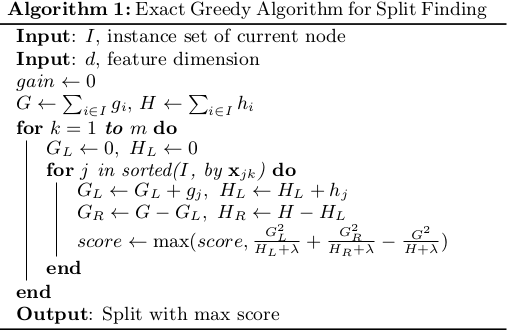
\includegraphics[width=0.7\linewidth]{img/exact_alg}
\caption{Split finding}
\label{fig:exact_alg}
\end{figure}	
\end{frame}

\end{document}
